\chapter{核苷酸与核酸}\label{ch:b1:nucleic-acids}

向破碎\omterm{def:b1:cell-unit-of-life:cell}{细胞}的溶液中加入冷乙醇，析出一团白色
絮状纤维，可用玻璃棒缠绕起来：\omterm{def:b1:nucleic-acids:chain}{DNA}，
即携带\omterm{def:b1:organism-environment:organism}{生物体}全部指令的分子，肉眼即可看见。
每个人类\omterm{def:b1:eukaryotic-cell:nucleus}{细胞核}中都折叠着两米长的 \omterm{def:b1:nucleic-acids:chain}{DNA}；其全部
信息以由四个字母组成的字母表书写，沿一个方向读取，
通过分开两条相互契合的链进行复制，二者如同
手与手套。本章介绍\omterm{def:b1:nucleic-acids:nucleotide}{核苷酸}——它们既是字母，
又是\omterm{def:b1:water-small-molecules:atp}{能量通货}和辅酶——以及它们构成的链、
\omterm{thm:b1:nucleic-acids:helix}{双螺旋}结构及其证据、\omterm{def:b1:nucleic-acids:chain}{DNA} 受热解链与复性的过程，
以及将遗传信息带入\omterm{def:b1:cell-unit-of-life:cell}{细胞}的 \omterm{def:b1:nucleic-acids:chain}{RNA}。

\section{核苷酸}

\begin{definition}[核苷酸]\label{def:b1:nucleic-acids:nucleotide}
\emph{核苷酸}\index{核苷酸}由三部分组成：一个含氮
\emph{碱基}\index{碱基}——即
\emph{嘌呤}\index{嘌呤}（腺嘌呤 A、鸟嘌呤 G：两个稠合的环）或
\emph{嘧啶}\index{嘧啶}（胞嘧啶 C、胸腺嘧啶 T、尿嘧啶 U：一个环）；
一种五碳糖，在 \omterm{def:b1:nucleic-acids:chain}{RNA} 中为\emph{核糖}，
在 \omterm{def:b1:nucleic-acids:chain}{DNA} 中为\emph{2$'$-脱氧核糖}（
缺少 $2'$ 位碳上的羟基）；以及连接在糖的 $5'$ 碳上的一至三个\emph{磷酸基团}。
碱基连接在 $1'$ 碳上；糖的碳原子
用撇号标号，以与碱基的编号相区别。碱基加
糖即为\emph{核苷}（腺苷、鸟苷、胞苷、
胸苷、尿苷）；加上磷酸基团即为核苷酸（AMP、ADP、\omterm{def:b1:water-small-molecules:atp}{ATP}
及其同类）。
\end{definition}

\begin{omfigure}
\begin{tikzpicture}[font=\footnotesize, line cap=round, line join=round]
  % phosphates
  \foreach \i/\c in {0/omThm!15,1/omThm!25,2/omThm!35} {
    \draw[thick, omThm!80!black, fill=\c, rounded corners=3pt] (1.3*\i,0.9) rectangle (1.3*\i+1.1,1.9);
    \node at (1.3*\i+0.55,1.4) {$\mathrm{P}$};
  }
  \node[anchor=south, align=center] at (1.65,2.15) {磷酸基团：$\gamma$、$\beta$、$\alpha$\\（它们之间为酸酐键）};
  \draw[thick] (3.3,1.4) -- (4.0,1.4);
  % sugar pentagon
  \draw[thick, omDef!80!black, fill=omDef!15] (4.0,1.4) -- (4.55,2.05) -- (5.45,2.05) -- (6.0,1.4) -- (5.0,0.85) -- cycle;
  \node at (5.0,1.5) {核糖};
  \node[font=\scriptsize] at (3.85,1.15) {$5'$};
  \node[font=\scriptsize] at (4.55,2.25) {$4'$};
  \node[font=\scriptsize] at (5.45,2.25) {$1'$};
  \node[font=\scriptsize] at (6.15,1.15) {$2'$};
  \node[font=\scriptsize] at (5.0,0.6) {$3'$};
  \draw[thick] (5.0,0.85) -- (5.0,0.2) node[below] {OH};
  \draw[thick] (6.0,1.4) -- (6.6,1.0) node[right] {OH（脱氧核糖中为 H）};
  % base
  \draw[thick] (5.45,2.05) -- (5.9,2.7);
  \draw[thick, omExo!80!black, fill=omExo!15, rounded corners=3pt] (5.4,2.7) rectangle (7.6,3.7);
  \node at (6.5,3.2) {碱基（A、G、C、U/T）};
  \node[anchor=west, align=left, gray] at (8.2,3.0) {核苷 = 碱基 + 糖 \\ 核苷酸 = 核苷 + 磷酸基团 \\ ATP = 腺嘌呤 + 核糖 + 三个磷酸基团};
\end{tikzpicture}

{\small \omterm{def:b1:nucleic-acids:nucleotide}{核苷酸}的组成：\omterm{def:b1:nucleic-acids:nucleotide}{碱基}连接在戊糖的 $1'$ 碳上，
磷酸基团连接在 $5'$ 碳上。$3'$ 位羟基是
链上下一个\omterm{def:b1:nucleic-acids:nucleotide}{核苷酸}的连接位点；$2'$ 位区分
\omterm{def:b1:nucleic-acids:chain}{RNA}（OH）与 \omterm{def:b1:nucleic-acids:chain}{DNA}（H）。}
\end{omfigure}

\begin{proposition}[核苷酸的三种功能]\label{prop:b1:nucleic-acids:threejobs}
除作为 \omterm{def:b1:nucleic-acids:chain}{DNA} 和 \omterm{def:b1:nucleic-acids:chain}{RNA} 的单体外，\omterm{def:b1:nucleic-acids:nucleotide}{核苷酸}还是\omterm{def:b1:cell-unit-of-life:cell}{细胞}的
\emph{\omterm{def:b1:water-small-molecules:atp}{能量通货}}——\omterm{def:b1:water-small-molecules:atp}{ATP} 与 GTP，其\omterm{def:b1:water-small-molecules:atp}{磷酸酐键}
（见\cref{ch:b1:water-small-molecules}）为合成、运输与
运动供能；其\emph{辅酶}——$\mathrm{NAD^+}$、$\mathrm{NADP^+}$
与 FAD，它们在呼吸作用和光合作用中传递电子
（见\cref{ch:b1:respiration-fermentation}），以及辅酶 A，它携带
酰基；其\emph{信使}——环 AMP，它在\omterm{def:b1:cell-unit-of-life:cell}{细胞}内
传递激素信号。它们全都是腺\omterm{def:b1:nucleic-acids:nucleotide}{嘌呤}\omterm{def:b1:nucleic-acids:nucleotide}{核苷酸}，或以之为基础
构成的：拼写信息的同一分子，也为其
执行提供动力。
\end{proposition}

\section{多核苷酸链}

\begin{definition}[磷酸二酯键与极性]\label{def:b1:nucleic-acids:chain}
\omterm{def:b1:nucleic-acids:nucleotide}{核苷酸}连接形成\emph{多核苷酸}\index{多核苷酸}，
通过\emph{磷酸二酯键}\index{磷酸二酯键}：一个\omterm{def:b1:nucleic-acids:nucleotide}{核苷酸}的
$5'$ 碳上的磷酸基团，与下一个
\omterm{def:b1:nucleic-acids:nucleotide}{核苷酸}的 $3'$ 位羟基相连。因此，链具有糖–磷酸
\emph{骨架}，均一且带负电（每个磷酸带一个负电荷），
从中伸出\omterm{def:b1:nucleic-acids:nucleotide}{碱基}，形成序列；链还具有
方向性：一端为\emph{$5'$ 端}\index{$5'$ 端}，带有游离的
磷酸基团，另一端为\emph{$3'$ 端}\index{$3'$ 端}，带有游离的
羟基。序列以 $5' \to 3'$ 方向书写和阅读，该方向即
链的合成方向。\emph{DNA}\index{DNA}（脱氧核糖核酸）
使用脱氧核糖和\omterm{def:b1:nucleic-acids:nucleotide}{碱基} A、G、C、T；\emph{RNA}\index{RNA}
（核糖核酸）使用核糖和\omterm{def:b1:nucleic-acids:nucleotide}{碱基} A、G、C、U。
\end{definition}

\begin{omfigure}
\begin{tikzpicture}[font=\footnotesize, line cap=round]
  \foreach \i/\b in {0/A,1/C,2/G,3/T} {
    \draw[thick, omThm!80!black, fill=omThm!25, rounded corners=2pt] (0.3,-1.6*\i+0.15) rectangle (0.9,-1.6*\i+0.75);
    \node at (0.6,-1.6*\i+0.45) {P};
    \draw[thick, omDef!80!black, fill=omDef!15] (1.3,-1.6*\i-0.1) -- (1.6,-1.6*\i+0.3) -- (2.2,-1.6*\i+0.3) -- (2.5,-1.6*\i-0.1) -- (1.9,-1.6*\i-0.5) -- cycle;
    \node[font=\scriptsize] at (1.9,-1.6*\i-0.1) {糖};
    \draw[thick] (0.9,-1.6*\i+0.45) -- (1.3,-1.6*\i-0.1);
    \node[font=\scriptsize] at (1.2,-1.6*\i+0.4) {$5'$};
    \node[font=\scriptsize] at (2.0,-1.6*\i-0.75) {$3'$};
    \draw[thick] (2.2,-1.6*\i+0.3) -- (2.9,-1.6*\i+0.3);
    \draw[thick, omExo!80!black, fill=omExo!15, rounded corners=2pt] (2.9,-1.6*\i+0.0) rectangle (3.7,-1.6*\i+0.6);
    \node at (3.3,-1.6*\i+0.3) {\b};
  }
  \foreach \i in {0,1,2} { \draw[thick] (1.9,-1.6*\i-0.5) -- (0.6,-1.6*\i-0.85); }
  \node[anchor=east, align=right] at (0.1,0.9) {$5'$ 端：\\ 游离磷酸基团};
  \node[anchor=east, align=right] at (0.1,-5.5) {$3'$ 端：\\ 游离羟基};
  \draw[thick] (1.9,-5.3) -- (1.9,-5.7) node[below, font=\scriptsize] {OH};
  \draw[->, very thick, gray] (4.6,0.6) -- (4.6,-5.2) node[midway, right, align=left] {书写与阅读方向 \\ $5' \to 3'$：\\ 该链为 \\ $5'$-ACGT-$3'$};
  \draw[thick, omThm!80!black] (0.4,-0.9) -- (0.4,-1.3);
  \node[anchor=west, align=left, gray] at (7.4,-2.6) {骨架：糖与磷酸交替排列 \\ 每个磷酸带一个负电荷 \\ 碱基：可变部分 \\ 即序列};
\end{tikzpicture}

{\small 四\omterm{def:b1:nucleic-acids:nucleotide}{核苷酸}链。每个\omterm{def:b1:nucleic-acids:nucleotide}{核苷酸}的 $5'$ 磷酸
通过\omterm{def:b1:nucleic-acids:chain}{磷酸二酯
键}与上方\omterm{def:b1:nucleic-acids:nucleotide}{核苷酸}的 $3'$ 羟基相连；链从 $5'$ 端延伸至 $3'$ 端，\omterm{def:b1:nucleic-acids:nucleotide}{碱基}
悬挂于均一的骨架上。}
\end{omfigure}

\begin{example}[RNA 易碎，DNA 耐久]\label{ex:b1:nucleic-acids:fragile}
核糖的 $2'$ 羟基可以攻击相邻的\omterm{def:b1:nucleic-acids:chain}{磷酸二酯
键}。在温和碱液中，\omterm{def:b1:nucleic-acids:chain}{RNA} 数小时内即被水解为\omterm{def:b1:nucleic-acids:nucleotide}{核苷酸}，
而 \omterm{def:b1:nucleic-acids:chain}{DNA} 因无此羟基，可耐受碱液煮沸，并
已从数万年之久的\omterm{def:b1:body-plans-tissues:segments}{骨骼}中完整提取。\omterm{def:b1:nucleic-acids:chain}{RNA} 中的尿\omterm{def:b1:nucleic-acids:nucleotide}{嘧啶}
即无甲基的胸腺\omterm{def:b1:nucleic-acids:nucleotide}{嘧啶}；\omterm{def:b1:nucleic-acids:chain}{DNA} 采用胸腺\omterm{def:b1:nucleic-acids:nucleotide}{嘧啶}，以便
胞\omterm{def:b1:nucleic-acids:nucleotide}{嘧啶}会缓慢失去氨基而变为尿\omterm{def:b1:nucleic-acids:nucleotide}{嘧啶}，从而可以
被\omterm{prop:b1:water-small-molecules:weak}{识别}为受损并加以修复——\omterm{def:b1:nucleic-acids:chain}{DNA} 中的尿\omterm{def:b1:nucleic-acids:nucleotide}{嘧啶}总是
错误。
\end{example}

\section{双螺旋}

\begin{proposition}[查加夫规则]\label{prop:b1:nucleic-acids:chargaff}
\index{查加夫规则}
任何\omterm{def:b1:organism-environment:organism}{生物体}的 \omterm{def:b1:nucleic-acids:chain}{DNA} 中，腺\omterm{def:b1:nucleic-acids:nucleotide}{嘌呤}的含量与
胸腺\omterm{def:b1:nucleic-acids:nucleotide}{嘧啶}的含量相等，鸟\omterm{def:b1:nucleic-acids:nucleotide}{嘌呤}的含量与胞\omterm{def:b1:nucleic-acids:nucleotide}{嘧啶}的相等（$A = T$，
$G = C$，因此\omterm{def:b1:nucleic-acids:nucleotide}{嘌呤}数 $=$ \omterm{def:b1:nucleic-acids:nucleotide}{嘧啶}数），而比值 $(G + C)/(A + T)$
因物种而异（从 \qty{25}{\%} 到 \qty{75}{\%}
$G + C$）。
\end{proposition}
\begin{proof}[证据]
\omterm{prop:b1:nucleic-acids:chargaff}{查加夫}（1950 年）水解了多种生物的 \omterm{def:b1:nucleic-acids:chain}{DNA}，并通过色谱法分离
\omterm{def:b1:nucleic-acids:nucleotide}{碱基}，再依据各\omterm{def:b1:nucleic-acids:nucleotide}{碱基}的紫外吸收进行测定。
所有 \omterm{def:b1:nucleic-acids:chain}{DNA} 中这些相等关系均在实验误差范围内成立；
$G + C$ 含量则并非如此，它在同一生物的每种\omterm{def:b1:body-plans-tissues:tissue}{组织}中
都相同。
\end{proof}

\begin{theorem}[沃森–克里克双螺旋]\label{thm:b1:nucleic-acids:helix}
\index{双螺旋}\index{碱基对}\index{反向平行}
\omterm{def:b1:nucleic-acids:chain}{DNA} 是两条\omterm{def:b1:nucleic-acids:chain}{多核苷酸}链绕同一轴盘绕成的
右手\emph{\omterm{thm:b1:nucleic-acids:helix}{双螺旋}}：糖–磷酸骨架位于
外侧，\omterm{def:b1:nucleic-acids:nucleotide}{碱基}位于内侧，呈平面状，并与轴垂直堆叠。
两条链呈\emph{反向平行}（一条沿 $5' \to 3'$ 向上，另一条
向下），并且\emph{互补}：与每个 A 相对的是 T，
二者以两个\omterm{def:b1:water-small-molecules:water}{氢键}相连；与每个 G 相对的是 C，以三个\omterm{def:b1:water-small-molecules:water}{氢键}相连；
每个这样的\emph{\omterm{thm:b1:nucleic-acids:helix}{碱基对}}宽度相同，因此螺旋
无论序列如何均匀一致。在常见的 B 型中，螺旋直径为 \qty{2}{nm}，
每个\omterm{thm:b1:nucleic-acids:helix}{碱基对}升高 \qty{0.34}{nm}，每圈十个\omterm{thm:b1:nucleic-acids:helix}{碱基对}升高
\qty{3.4}{nm}，并呈现宽的\emph{大沟}和窄的
\emph{小沟}，其中\omterm{def:b1:nucleic-acids:nucleotide}{碱基}边缘暴露，可与
蛋白质作用。
\end{theorem}
\begin{proof}[证据]
富兰克林（1952 年）的 \omterm{def:b1:nucleic-acids:chain}{DNA} 纤维 X 射线衍射照片显示出
螺旋的交叉图样，沿轴的重复周期为 \qty{3.4}{nm}，并有一个
位于 \qty{0.34}{nm} 处的强反射（对应平面堆叠单元），以及
\qty{2}{nm} 的直径；磷原子作为最重的原子，必须位于
外侧。沃森和克里克（1953 年）发现，一个\omterm{def:b1:nucleic-acids:nucleotide}{嘌呤}与一个\omterm{def:b1:nucleic-acids:nucleotide}{嘧啶}配对
——且仅 A 与 T、G 与 C 配对——所得\omterm{thm:b1:nucleic-acids:helix}{碱基对}宽度相等，
与 \qty{2}{nm} 的直径相符，并可解释\omterm{prop:b1:nucleic-acids:chargaff}{查加夫}规则；
两条反向平行链如此配对，构成规则螺旋，
其尺寸与纤维的测量结果一致。该模型预言每条链都是
另一条链的模板；梅塞尔森与斯塔尔关于
半保留复制的实验（回顾高中分册，
并见\cref{ch:b1:replication-mitosis}）证实了这一预言。
\end{proof}

\begin{omfigure}
\begin{minipage}[b]{0.34\linewidth}\centering
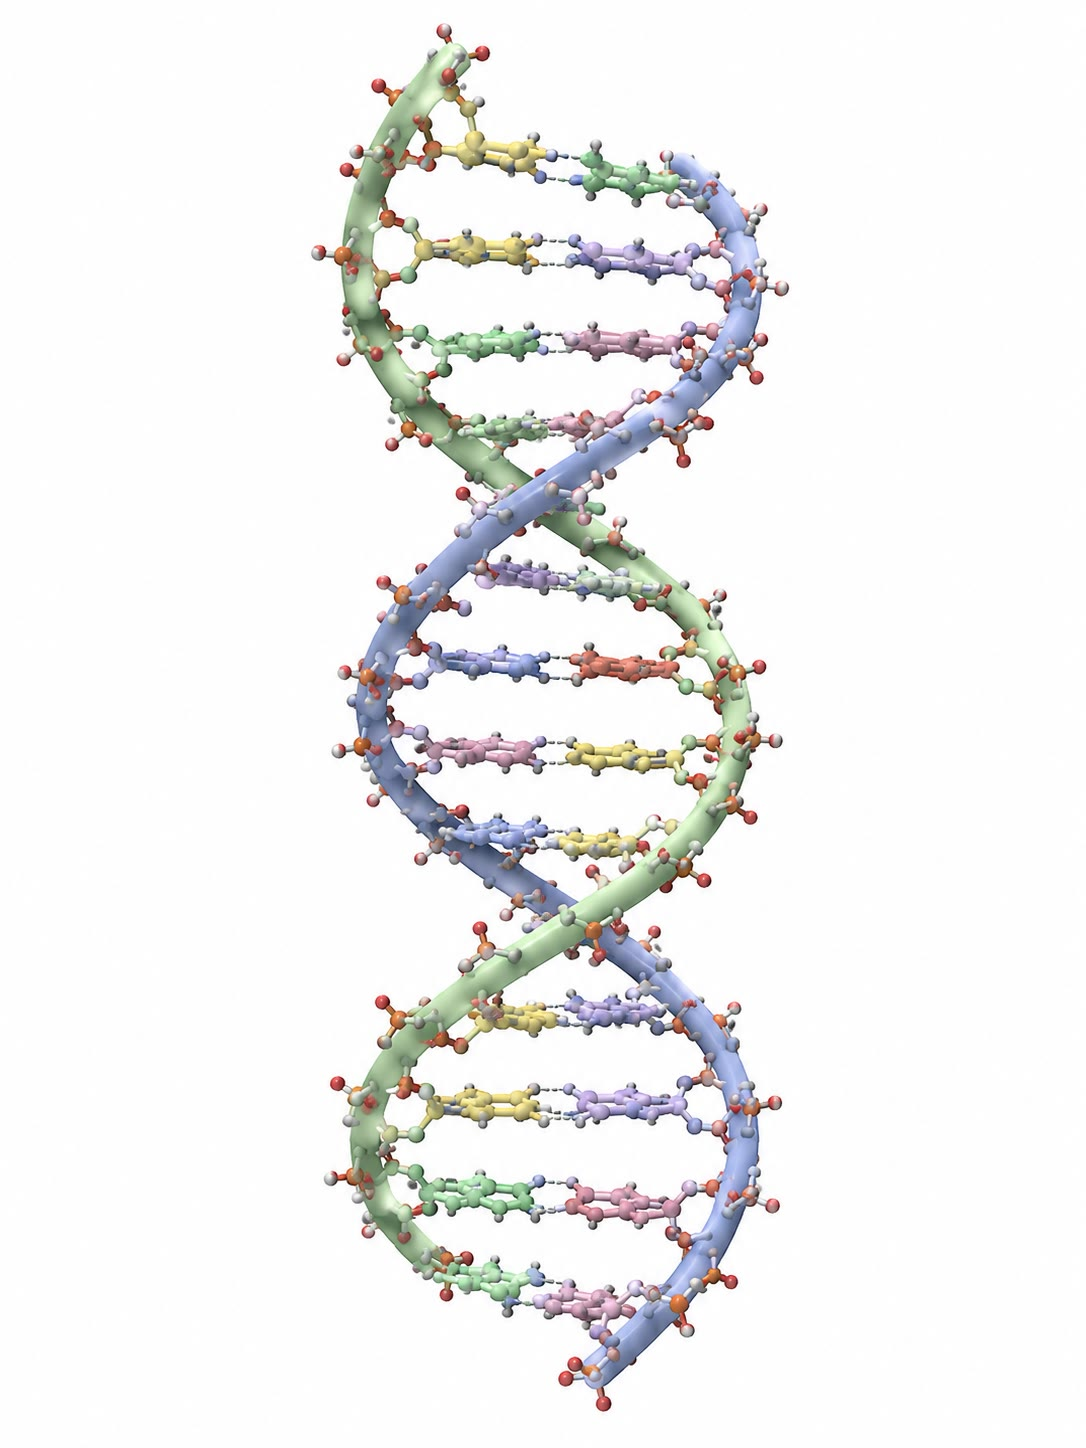
\includegraphics[width=0.9\linewidth]{images/book3/ai/fig-dna-double-helix.jpg}
\end{minipage}\hfill
\begin{minipage}[b]{0.62\linewidth}\centering
\begin{tikzpicture}[font=\footnotesize, line cap=round]
  % two antiparallel backbones as vertical bars, base pairs as rungs
  \draw[line width=3pt, omDef] (0,0) -- (0,5.1);
  \draw[line width=3pt, omDef!50] (2.6,0) -- (2.6,5.1);
  \foreach \i/\l/\r/\n in {0/A/T/2,1/G/C/3,2/T/A/2,3/C/G/3,4/A/T/2,5/G/C/3,6/C/G/3,7/T/A/2,8/G/C/3,9/A/T/2} {
    \pgfmathsetmacro{\y}{0.3+0.5*\i}
    \draw[thick, omExo!80!black, fill=omExo!20] (0.1,\y-0.14) rectangle (1.2,\y+0.14);
    \draw[thick, omExo!80!black, fill=omExo!20] (1.4,\y-0.14) rectangle (2.5,\y+0.14);
    \node[font=\scriptsize] at (0.65,\y) {\l}; \node[font=\scriptsize] at (1.95,\y) {\r};
    \ifnum\n=3 \draw[dashed] (1.2,\y-0.08) -- (1.4,\y-0.08) (1.2,\y) -- (1.4,\y) (1.2,\y+0.08) -- (1.4,\y+0.08);
    \else \draw[dashed] (1.2,\y-0.05) -- (1.4,\y-0.05) (1.2,\y+0.05) -- (1.4,\y+0.05); \fi
  }
  \node[anchor=south, omDef] at (0,5.15) {$5'$}; \node[anchor=north, omDef] at (0,-0.05) {$3'$};
  \node[anchor=south, omDef!70!black] at (2.6,5.15) {$3'$}; \node[anchor=north, omDef!70!black] at (2.6,-0.05) {$5'$};
  \draw[<->, thick] (3.2,0.3) -- (3.2,4.8) node[midway, right, align=left] {十个碱基对 \\ $= \qty{3.4}{nm}$\\ $=$ 一圈};
  \draw[<->, thick] (3.2,-0.6) -- (3.2,0.3) node[midway, right] {};
  \draw[<->, thick] (0,-0.9) -- (2.6,-0.9) node[midway, below] {\qty{2}{nm}};
  \draw[<->, thick] (-0.5,0.3) -- (-0.5,0.8) node[midway, left] {\qty{0.34}{nm}};
  \node[anchor=west, align=left, font=\scriptsize] at (3.2,5.2) {A--T：2 个氢键 \\ G--C：3 个氢键};
\end{tikzpicture}
\end{minipage}

{\small 左：\omterm{thm:b1:nucleic-acids:helix}{双螺旋}模型；两条骨架
环绕堆叠的\omterm{thm:b1:nucleic-acids:helix}{碱基对}盘绕，形成大沟与小沟。
右：同样的十个\omterm{thm:b1:nucleic-acids:helix}{碱基对}展开为梯状结构：反向平行
链，互补\omterm{thm:b1:nucleic-acids:helix}{碱基对}宽度相等，每对 \qty{0.34}{nm}，
每圈 \qty{3.4}{nm}。}
\end{omfigure}

\begin{example}[读取一条链]\label{ex:b1:nucleic-acids:complement}
若一条链为 $5'$-ATGGCATTC-$3'$，其互补链（按
$5' \to 3'$ 书写）为 $5'$-GAATGCCAT-$3'$：先逐个取互补\omterm{def:b1:nucleic-acids:nucleotide}{碱基}，再颠倒顺序。
共九个\omterm{thm:b1:nucleic-acids:helix}{碱基对}，螺旋长 \qty{3.1}{nm}，\omterm{def:b1:water-small-molecules:water}{氢键}
共二十二个（G--C 五个，A--T 四个）。一条含 \num{2.5e8} 个\omterm{thm:b1:nucleic-acids:helix}{碱基对}的人类染色体
在此形式下长 \qty{8.5}{cm}，必须折叠十万次，
方可装入\omterm{def:b1:eukaryotic-cell:nucleus}{细胞核}（见\cref{ch:b1:genomes}）。
\end{example}

\begin{proposition}[维系双螺旋的因素]\label{prop:b1:nucleic-acids:stability}
配对\omterm{def:b1:nucleic-acids:nucleotide}{碱基}之间的\omterm{def:b1:water-small-molecules:water}{氢键}提供专一性；平面\omterm{def:b1:nucleic-acids:nucleotide}{碱基}
彼此叠放形成的\emph{堆积}\index{碱基堆积}
——\omterm{def:b1:water-small-molecules:bonds}{范德华}接触与使\omterm{def:b1:nucleic-acids:nucleotide}{碱基}远离水的\omterm{prop:b1:water-small-molecules:properties}{疏水效应}——
提供了大部分稳定性；带负电荷的
骨架彼此排斥，\omterm{thm:b1:nucleic-acids:helix}{双螺旋}只有在
存在阳离子（生理条件下的 $\mathrm{Mg^{2+}}$、
$\mathrm{Na^+}$，或\omterm{def:b1:eukaryotic-cell:nucleus}{染色质}中的碱性蛋白）时才稳定，
它们屏蔽了电荷。G--C \omterm{thm:b1:nucleic-acids:helix}{碱基对}具有三个\omterm{def:b1:water-small-molecules:water}{氢键}、\omterm{prop:b1:nucleic-acids:stability}{堆积}作用更强，
比 A--T \omterm{thm:b1:nucleic-acids:helix}{碱基对}更稳定。
\end{proposition}

\section{解链与杂交}

\begin{definition}[变性，解链温度]\label{def:b1:nucleic-acids:melting}
加热或极端的 \omterm{def:b1:water-small-molecules:ph}{pH} 会使 \omterm{def:b1:nucleic-acids:chain}{DNA} 的两条链分开：
\emph{变性}\index{变性 (DNA)}（熔解）是一种协同
转变，在几度范围内完成，其中点即为\emph{解链温度}\index{解链温度}
$T_m$。随后出现
\emph{增色效应}：单链在 \qty{260}{nm} 处的紫外吸收约高 \qty{40}{\%}，
比同样\omterm{def:b1:nucleic-acids:nucleotide}{碱基}在螺旋中堆叠时更强。
$T_m$ 随 $G + C$ 含量升高（每百分比约 \qty{0.4}{\celsius}
），也随盐浓度和长度升高；在
\qty{0.15}{mol/L} 盐溶液中，$G + C$ 含量为 \qty{50}{\%} 的长 \omterm{def:b1:nucleic-acids:chain}{DNA} 在 \qty{90}{\celsius} 附近解链。
缓慢冷却后，两条链找到各自的互补链，
并重新形成螺旋：\emph{复性}，若两条链来自不同来源，
则称为\emph{杂交}\index{杂交}。
\end{definition}

\begin{omfigure}
\begin{tikzpicture}
\begin{axis}[
  width=0.86\linewidth, height=6.0cm,
  axis x line=bottom, axis y line=left,
  xmin=60, xmax=105, ymin=0.95, ymax=1.5,
  xlabel={温度 (\unit{\celsius})}, ylabel={\qty{260}{nm} 处的相对吸光度},
  xlabel style={font=\small, at={(axis description cs:0.5,-0.12)}, anchor=north},
  ylabel style={font=\small},
  tick label style={font=\small}, xtick={60,70,80,90,100}, ytick={1.0,1.2,1.4},
  legend style={font=\small, at={(0.03,0.97)}, anchor=north west, draw=none},
  clip=false,
]
\addplot[very thick, omDef, domain=60:105, samples=120] {1+0.4/(1+exp(-(x-77)/1.5))};
\addlegendentry{\qty{30}{\%} $G+C$：$T_m = \qty{77}{\celsius}$}
\addplot[very thick, omThm, domain=60:105, samples=120] {1+0.4/(1+exp(-(x-93)/1.5))};
\addlegendentry{\qty{70}{\%} $G+C$：$T_m = \qty{93}{\celsius}$}
\draw[dashed, gray] (axis cs:60,1.2) -- (axis cs:93,1.2);
\draw[dashed, gray] (axis cs:77,0.95) -- (axis cs:77,1.2);
\draw[dashed, gray] (axis cs:93,0.95) -- (axis cs:93,1.2);
\end{axis}
\end{tikzpicture}

{\small 同一盐溶液中两种 \omterm{def:b1:nucleic-acids:chain}{DNA} 的解链曲线。吸光度
随链分离在几度范围内上升 \qty{40}{\%}；其中点
$T_m$ 对富含 G--C \omterm{thm:b1:nucleic-acids:helix}{碱基对}的 \omterm{def:b1:nucleic-acids:chain}{DNA} 更高。}
\end{omfigure}

\begin{method}[用吸光度测定核酸]\label{met:b1:nucleic-acids:absorbance}
\begin{enumerate}
  \item \omterm{def:b1:nucleic-acids:nucleotide}{碱基}在紫外区有吸收，最大吸收峰位于
        \qty{260}{nm} 处。在 \qty{1}{cm} 光程的比色皿中，吸光度 $1.0$
        相当于 \qty{50}{\micro g/mL} 的双链 \omterm{def:b1:nucleic-acids:chain}{DNA}，
        （\omterm{def:b1:nucleic-acids:chain}{RNA} 为 \qty{40}{\micro g/mL}，
        单链 \omterm{def:b1:nucleic-acids:chain}{DNA} 为 \qty{33}{\micro g/mL}）。
  \item 纯 \omterm{def:b1:nucleic-acids:chain}{DNA} 的比值 $A_{260}/A_{280}$ 为 $1.8$，
        纯 \omterm{def:b1:nucleic-acids:chain}{RNA} 为 $2.0$；蛋白质在 \qty{280}{nm} 处有吸收，会使比值降低。
  \item 若要跟踪解链，在缓慢加热的同时记录 $A_{260}$；
        曲线的中点即为 $T_m$，其陡峭程度衡量样品的
        均一性。
  \item 若要检测某一序列，先使样品\omterm{def:b1:nucleic-acids:melting}{变性}，再加入与之互补的带标记单链
        （即\emph{探针}）；探针只在互补序列所在之处\omterm{def:b1:nucleic-acids:melting}{杂交}，
        标记则指明其位置
        ——在凝胶上、在染色体上，或在\omterm{def:b1:body-plans-tissues:tissue}{组织}中。
\end{enumerate}
\end{method}

\begin{omfigure}
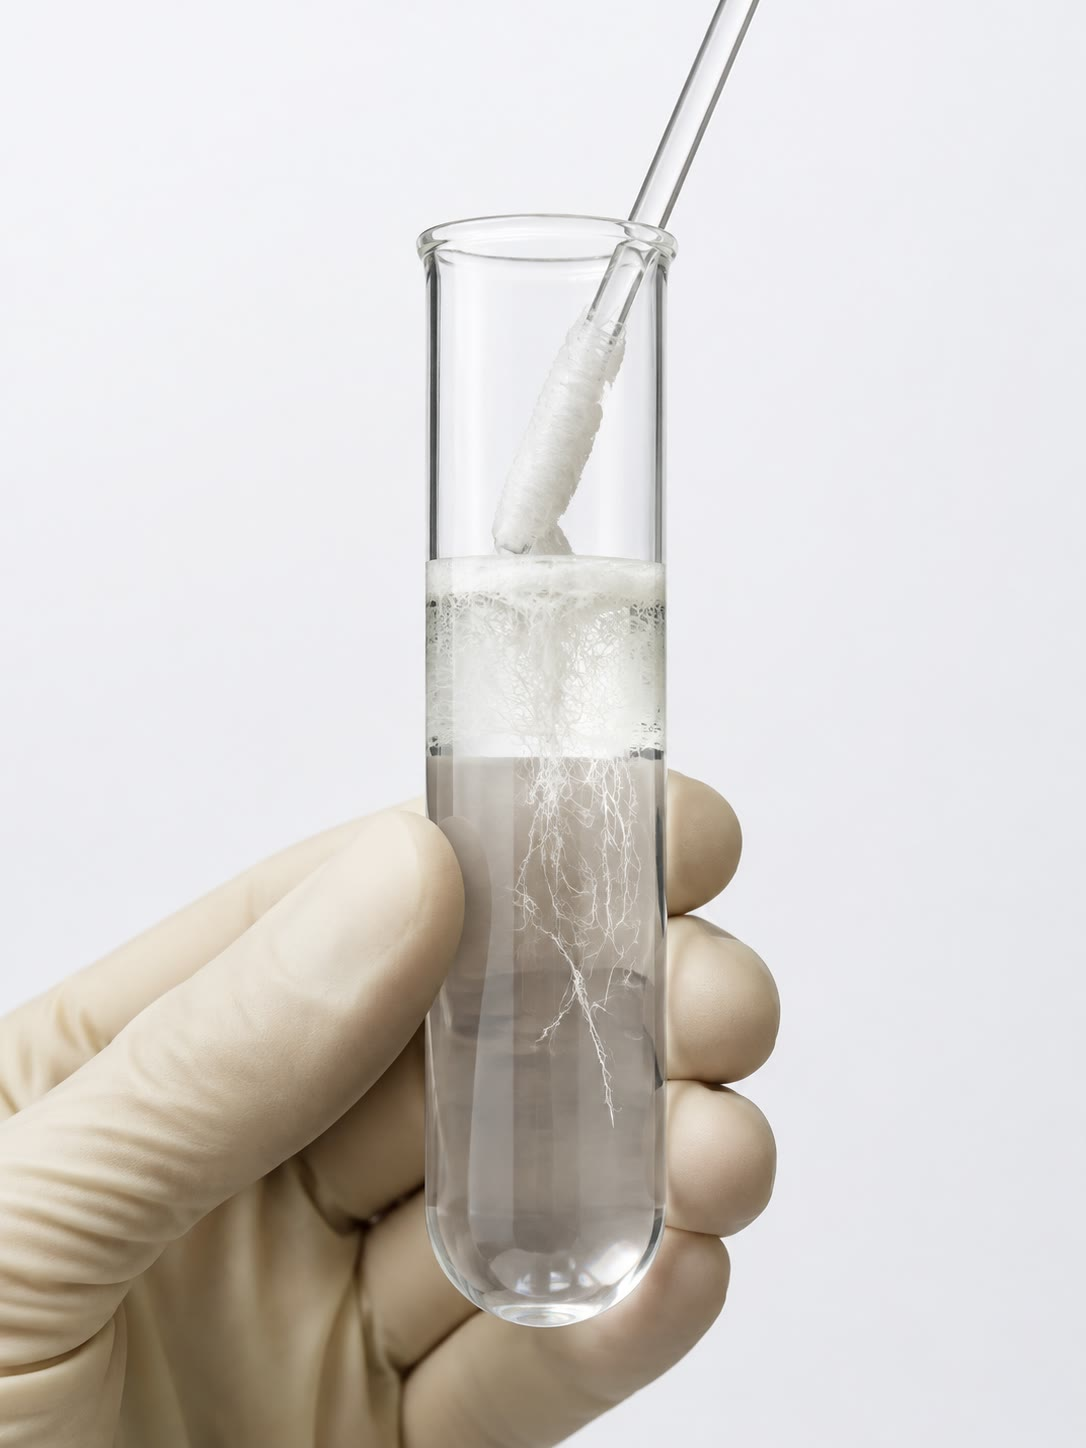
\includegraphics[width=0.3\linewidth]{images/book3/ai/b3-11-dna-precipitate.jpg}

{\small 从\omterm{def:b1:cell-unit-of-life:cell}{细胞}裂解物中用冷乙醇沉淀出的 \omterm{def:b1:nucleic-acids:chain}{DNA}，缠绕在玻璃棒上：
约几毫克的分子，肉眼可见为纤维状，
因每条分子长达数百万个\omterm{thm:b1:nucleic-acids:helix}{碱基对}。}
\end{omfigure}

\begin{example}[探针寻找基因]\label{ex:b1:nucleic-acids:probe}
一条与某一基因互补的二十\omterm{def:b1:nucleic-acids:nucleotide}{核苷酸}探针，在
低于其自身 $T_m$ \qty{5}{\celsius} 的条件下，只与其精确互补序列结合，
在三十亿个\omterm{thm:b1:nucleic-acids:helix}{碱基对}中不与其他任何序列结合：二十个\omterm{def:b1:nucleic-acids:nucleotide}{碱基}中只要有一处错配，
$T_m$ 降低数度，错配的\omterm{def:b1:nucleic-acids:melting}{杂交}链便会解链。
\omterm{def:b1:nucleic-acids:nucleotide}{碱基}配对的专一性在二十个位点上相乘，正是
从亲子鉴定到病原体检测，一切 \omterm{def:b1:nucleic-acids:chain}{DNA} 检测所依赖的基础。
\end{example}

\section{RNA 分子}

\begin{definition}[各类 RNA]\label{def:b1:nucleic-acids:rnas}
\omterm{def:b1:nucleic-acids:chain}{RNA} 通常为单链，凡短的互补片段允许之处，便会折叠回自身，
形成发夹、环和凸起，
——即\emph{二级结构}——再进一步\omterm{prop:b1:nucleic-acids:stability}{堆积}成一定的形状。
三类 \omterm{def:b1:nucleic-acids:chain}{RNA} 承载着遗传信息的流动
（见\cref{ch:b1:gene-expression}）：\emph{信使 RNA}\index{信使 RNA}（mRNA），即核糖体所读取的基因拷贝；
\emph{转运 RNA}\index{转运 RNA}（tRNA），约 \qty{75}{} 个\omterm{def:b1:nucleic-acids:nucleotide}{核苷酸}
折叠成三叶草形，在其
$3'$ 端携带一个氨基酸，并带有与信使 \omterm{def:b1:nucleic-acids:chain}{RNA} 配对的\emph{反密码子}；
\emph{核糖体 RNA}\index{核糖体 RNA}（rRNA），是核糖体的结构和
催化核心，占\omterm{def:b1:cell-unit-of-life:cell}{细胞} \omterm{def:b1:nucleic-acids:chain}{RNA} 的五分之四。
还有许多其他 \omterm{def:b1:nucleic-acids:chain}{RNA} 参与调控、剪接和引导（见本科三年级分册）。
\end{definition}

\begin{omfigure}
\begin{tikzpicture}[font=\footnotesize, line cap=round, >=Stealth]
  % acceptor stem (vertical, top)
  \draw[line width=2.5pt, omDef] (0,0) -- (0,2.2);
  \draw[line width=2.5pt, omDef] (0.5,0) -- (0.5,2.2);
  \foreach \y in {0.3,0.65,1.0,1.35,1.7} { \draw[thick, omExo!80!black] (0,\y) -- (0.5,\y); }
  \node[anchor=south] at (0,2.25) {$5'$};
  \draw[line width=2.5pt, omDef] (0.5,2.2) -- (0.5,2.9) -- (1.0,3.2);
  \node[anchor=west] at (1.0,3.2) {$3'$-CCA：氨基酸连接于此};
  % D arm (left)
  \draw[line width=2.5pt, omDef] (0,0) -- (-1.4,0) (0,-0.5) -- (-1.4,-0.5);
  \foreach \x in {-0.3,-0.65,-1.0} { \draw[thick, omExo!80!black] (\x,0) -- (\x,-0.5); }
  \draw[line width=2.5pt, omDef] (-1.4,0) arc (90:270:0.25);
  \node[anchor=east, align=right] at (-1.8,-0.25) {D 臂};
  % T arm (right)
  \draw[line width=2.5pt, omDef] (0.5,0) -- (1.9,0) (0.5,-0.5) -- (1.9,-0.5);
  \foreach \x in {0.8,1.15,1.5} { \draw[thick, omExo!80!black] (\x,0) -- (\x,-0.5); }
  \draw[line width=2.5pt, omDef] (1.9,0) arc (90:-90:0.25);
  \node[anchor=west, align=left] at (2.3,-0.25) {T 臂};
  % anticodon stem (down)
  \draw[line width=2.5pt, omDef] (0,-0.5) -- (0,-2.2) (0.5,-0.5) -- (0.5,-2.2);
  \foreach \y in {-0.85,-1.2,-1.55,-1.9} { \draw[thick, omExo!80!black] (0,\y) -- (0.5,\y); }
  \draw[line width=2.5pt, omDef] (0,-2.2) arc (180:360:0.25);
  \foreach \x in {0.1,0.25,0.4} { \fill[omThm] (\x,-2.5) circle (0.06); }
  \node[anchor=north, align=center] at (0.25,-2.65) {反密码子环：三个碱基 \\与 mRNA 的密码子配对};
  \node[anchor=west, align=left, gray] at (2.3,1.2) {四段配对碱基茎 \\（三叶草形），在三维空间中 \\折叠成 L 形};
\end{tikzpicture}

{\small 转运 \omterm{def:b1:nucleic-acids:chain}{RNA} 的三叶草形二级结构：一条
约 75 个\omterm{def:b1:nucleic-acids:nucleotide}{核苷酸}的单链自身配对，形成四段
茎。氨基酸携带在 $3'$ 端，反密码子位于
另一端，读取信息。}
\end{omfigure}

\begin{remark}[RNA 也可以是催化剂]\label{rem:b1:nucleic-acids:ribozyme}
部分 \omterm{def:b1:nucleic-acids:chain}{RNA} 是酶（\emph{核酶}）：每一种
蛋白质的肽键由核糖体 \omterm{def:b1:nucleic-acids:chain}{RNA} 形成，而非由蛋白质形成，还有些
\omterm{def:b1:nucleic-acids:chain}{RNA} 能自我切割和拼接。一种分子若既携带
信息又催化反应，可能正是最初生命系统
的构成物质；\omterm{def:b1:nucleic-acids:chain}{DNA} 与蛋白质的世界则是
较晚的一种分工，\omterm{def:b1:nucleic-acids:chain}{RNA} 仍居于其中心。
\end{remark}

\section{练习}

\begin{exercise}[$\star$]\label{exo:b1:nucleic-acids:1}
说出\omterm{def:b1:nucleic-acids:nucleotide}{核苷酸}的三个组成部分，以及核糖\omterm{def:b1:nucleic-acids:nucleotide}{核苷酸}
与脱氧核糖\omterm{def:b1:nucleic-acids:nucleotide}{核苷酸}之间的两点区别。
\end{exercise}

\begin{exercise}[$\star$]\label{exo:b1:nucleic-acids:2}
写出 $5'$-GGATCCTA-$3'$ 的互补链，并按 $5' \to 3'$
方向书写，并计算其\omterm{def:b1:water-small-molecules:water}{氢键}数。
\end{exercise}

\begin{exercise}[$\star$]\label{exo:b1:nucleic-acids:3}
一段 \omterm{def:b1:nucleic-acids:chain}{DNA} 含 \qty{22}{\%} 的腺\omterm{def:b1:nucleic-acids:nucleotide}{嘌呤}。求 T、G 和
C 的百分比，以及 $G + C$ 含量。
\end{exercise}

\begin{exercise}[$\star$]\label{exo:b1:nucleic-acids:4}
由解链图，求 $T_m$ 为多少的 \omterm{def:b1:nucleic-acids:chain}{DNA}，其
$G + C$ 含量为 \qty{50}{\%}，在相同条件下，
解链时吸光度升高多少？
\end{exercise}

\begin{exercise}[$\star\star$]\label{exo:b1:nucleic-acids:5}
计算 \emph{E. coli} 染色体的长度（$\num{4.6e6}$
\omterm{thm:b1:nucleic-acids:helix}{碱基对}），以毫米为单位，求其螺旋圈数，以及
需压缩的倍数，使其能装入一个 \qty{2}{\micro m} 的\omterm{def:b1:cell-unit-of-life:cell}{细胞}。
\end{exercise}

\begin{exercise}[$\star\star$]\label{exo:b1:nucleic-acids:6}
解释为何 \omterm{def:b1:nucleic-acids:chain}{DNA} 的两条链必须反向平行，并利用
糖–磷酸骨架的几何结构，以及每个\omterm{thm:b1:nucleic-acids:helix}{碱基对}宽度
须相同这一要求加以说明。
\end{exercise}

\begin{exercise}[$\star\star$]\label{exo:b1:nucleic-acids:7}
一份 \omterm{def:b1:nucleic-acids:chain}{DNA} 溶液在 \qty{1}{cm} 比色皿中，$A_{260} = 0.35$，
$A_{280} = 0.20$。求其浓度，并评论其纯度。
\qty{1}{mL} 中有多少个\omterm{thm:b1:nucleic-acids:helix}{碱基对}？若每个\omterm{thm:b1:nucleic-acids:helix}{碱基对}的
平均质量为 \qty{650}{Da}？
\end{exercise}

\begin{exercise}[$\star\star$]\label{exo:b1:nucleic-acids:8}
解释增色效应，并说明为何纯 \omterm{def:b1:nucleic-acids:chain}{DNA} 的解链曲线陡峭，
而来自多个物种的 \omterm{def:b1:nucleic-acids:chain}{DNA} 混合物则
\omterm{def:b1:nucleic-acids:melting}{解链温度}范围较宽。
\end{exercise}

\begin{exercise}[$\star\star$]\label{exo:b1:nucleic-acids:9}
一条二十\omterm{def:b1:nucleic-acids:nucleotide}{核苷酸}的探针，与其完全互补序列配对时 $T_m = \qty{62}{\celsius}$，
一个错配使 $T_m$ 降低约 \qty{5}{\celsius}。在
哪一温度下进行\omterm{def:b1:nucleic-acids:melting}{杂交}，才能检测到精确的
序列并排除单个错配？
\qty{45}{\celsius} 时会发生什么？
\end{exercise}

\begin{exercise}[$\star\star\star$]\label{exo:b1:nucleic-acids:10}
\omterm{prop:b1:nucleic-acids:chargaff}{查加夫}规则适用于双链 \omterm{def:b1:nucleic-acids:chain}{DNA}，但不适用于 \omterm{def:b1:nucleic-acids:chain}{RNA} 或
某些小型病毒的 \omterm{def:b1:nucleic-acids:chain}{DNA}。解释每种例外说明了
这些核酸结构的哪些特点。
\end{exercise}

\begin{exercise}[$\star\star\star$]\label{exo:b1:nucleic-acids:11}
两个\omterm{def:b1:water-small-molecules:water}{氢键}维系一个 A--T \omterm{thm:b1:nucleic-acids:helix}{碱基对}，然而由一千个 A--T
\omterm{thm:b1:nucleic-acids:helix}{碱基对}组成的螺旋在 \qty{60}{\celsius} 时稳定，而单个\omterm{thm:b1:nucleic-acids:helix}{碱基对}
根本不能形成。请用在\cref{ch:b1:water-small-molecules}中的
概念（弱键、协同性、\omterm{prop:b1:nucleic-acids:stability}{堆积}）加以解释，并说明
这对探针的保真度有何意义。
\end{exercise}

\begin{exercise}[$\star\star\star$]\label{exo:b1:nucleic-acids:12}
“\omterm{def:b1:nucleic-acids:chain}{DNA} 的结构即是遗传的解释。”用一段文字讨论：
\omterm{thm:b1:nucleic-acids:helix}{双螺旋}结构直接解释了哪些问题（复制、
作为序列改变的突变），哪些问题它本身无法解释
（序列如何变为蛋白质），以及为何沃森和克里克的模型
在对其进行任何生化检验之前就已被接受。
\end{exercise}

\section{问题：一种病毒的基因组}

\begin{problem}[{周末问题——噬菌体 $\lambda$ 的 DNA
经测量、称重、计数、解链并装入其衣壳，最后
归结到解链温度与轮廓长度}]
\label{pb:b1:nucleic-acids:1}
噬菌体 $\lambda$ 的基因组是一条线性双链 \omterm{def:b1:nucleic-acids:chain}{DNA}，
含 \num{48502} 个\omterm{thm:b1:nucleic-acids:helix}{碱基对}，$G + C$ 含量为 \qty{49.9}{\%}。它
装在一个内径为 \qty{55}{nm} 的二十面体衣壳中。
取每个\omterm{thm:b1:nucleic-acids:helix}{碱基对} \qty{0.34}{nm}，螺旋
直径 \qty{2.0}{nm}，每个\omterm{thm:b1:nucleic-acids:helix}{碱基对} \qty{650}{Da}，并取 $T_m = 81.5 + 16.6\log_{10}[\mathrm{Na^+}]
+ 0.41\,(\%\,G{+}C) - 500/L$（单位为摄氏度），其中 $[\mathrm{Na^+}]$
以 \unit{mol/L} 为单位，$L$ 为以\omterm{thm:b1:nucleic-acids:helix}{碱基对}计的长度。

\medskip
\noindent\textbf{第一部分——测量与称重。}
\begin{enumerate}
  \item 以微米为单位，计算该分子的轮廓长度。
  \item 计算螺旋的圈数。
  \item 以道尔顿为单位，计算其摩尔质量。
  \item 以克为单位，计算一个分子的质量。
  \item 计算磷酸基团的数目，并由此求出
        该分子的净电荷。
  \item 计算每种\omterm{def:b1:nucleic-acids:nucleotide}{碱基}（A、T、G、C）的\omterm{def:b1:nucleic-acids:nucleotide}{核苷酸}数目。
  \item 计算维系两条链的
        \omterm{def:b1:water-small-molecules:water}{氢键}总数。
\end{enumerate}

\medskip
\noindent\textbf{第二部分——已熔化。}
\begin{enumerate}[resume]
  \item 在 \qty{0.1}{mol/L} 钠盐溶液中计算 $T_m$。
  \item 在 \qty{0.01}{mol/L} 钠盐溶液中计算 $T_m$，
        并解释盐为何能稳定\omterm{thm:b1:nucleic-acids:helix}{双螺旋}。
  \item $\lambda$ 基因组中有一段含 \qty{1000}{} 个\omterm{thm:b1:nucleic-acids:helix}{碱基对}的区域，
        其 $G + C$ 含量为 \qty{35}{\%}，另一段为 \qty{62}{\%}。计算两段区域的
        $T_m$，溶液为 \qty{0.1}{mol/L} 钠盐，并描述
        整个分子熔解曲线的形状。
  \item 一份 $\lambda$ \omterm{def:b1:nucleic-acids:chain}{DNA} 溶液在熔解前 $A_{260} = 0.50$，
        其浓度是多少，完全熔解后的 $A_{260}$
        将为多少？
  \item \qty{1}{mL} 该溶液中含有
        多少个 $\lambda$ 分子？
  \item $\lambda$ 基因组的两端为单链突出端，
        各含 12 个\omterm{def:b1:nucleic-acids:nucleotide}{核苷酸}，彼此互补，分子借此在宿主中环化。
        计算它们的
        $T_m$（取 $L = 12$），并说明为何环状分子仍能保持
        在\omterm{def:b1:cell-unit-of-life:cell}{细胞}内 \qty{37}{\celsius} 时稳定。
\end{enumerate}

\medskip
\noindent\textbf{第三部分——已装填。}
\begin{enumerate}[resume]
  \item 将 \omterm{def:b1:nucleic-acids:chain}{DNA} 视为圆柱体，计算其体积。
  \item 计算衣壳的内部体积。
  \item \omterm{def:b1:nucleic-acids:chain}{DNA} 占据衣壳的比例是多少？与
        平行圆柱体的最紧密\omterm{prop:b1:nucleic-acids:stability}{堆积}（\qty{91}{\%}）作比较。
  \item \omterm{def:b1:nucleic-acids:chain}{DNA} 在一个 \qty{55}{nm} 的球体内
        带有 \num{97000} 个负电荷。请解释哪些物质必须随 \omterm{def:b1:nucleic-acids:chain}{DNA} 进入
        衣壳，以及为何被装填的 \omterm{def:b1:nucleic-acids:chain}{DNA} 会对外壳产生压强
        （数十个大气压），从而有助于将其注入细菌。
  \item 分子必须弯曲成半径与
        衣壳相当的环。\omterm{def:b1:nucleic-acids:chain}{DNA} 在半径约小于
        \qty{50}{nm} 时难以弯曲，对此加以评论。
\end{enumerate}

\medskip
\noindent\textbf{第四部分——读取。}
\begin{enumerate}[resume]
  \item 基因组的一条链以 $5'$-GGGCGGCGACCT-$3'$ 开始。写出
        与之互补的链（$5' \to 3'$）。
  \item 若一个含 \num{1200} 个\omterm{thm:b1:nucleic-acids:helix}{碱基对}的基因被转录为 mRNA，
        则该 mRNA 的长度是多少个\omterm{def:b1:nucleic-acids:nucleotide}{核苷酸}，并
        若每个\omterm{def:b1:nucleic-acids:nucleotide}{核苷酸}为 \qty{330}{Da}，其质量为多少？
  \item 该基因组含 \qty{75}{} 个基因，共 \num{48502} 个\omterm{thm:b1:nucleic-acids:helix}{碱基对}。若平均每个基因为
        \num{600} 个\omterm{thm:b1:nucleic-acids:helix}{碱基对}，则编码部分占基因组的比例是多少？
        与人类基因组（\qty{1.5}{\%}）作比较。
  \item 该基因组在 \qty{37}{\celsius} 下，于 \qty{20}{min} 内
        由宿主的酶完成复制。计算以每秒\omterm{thm:b1:nucleic-acids:helix}{碱基对}计的复制速率，
        若复制从一个复制起点开始，并沿
        两个方向进行。
  \item 复制期间两个复制叉处每秒有多少个\omterm{def:b1:water-small-molecules:water}{氢键}被断开
        （取问题
        7 中每个\omterm{thm:b1:nucleic-acids:helix}{碱基对}的平均值）？
  \item 一次突变将一个 G--C \omterm{thm:b1:nucleic-acids:helix}{碱基对}变为 A--T。整个分子的
        $T_m$ 改变了多少？熔解能否检测出这一突变？
  \item 给出结果：$\lambda$ \omterm{def:b1:nucleic-acids:chain}{DNA} 的熔解温度（在
        \qty{0.1}{mol/L} 钠盐中）、其轮廓长度，以及
        使其装入衣壳所需的压缩程度。
\end{enumerate}
\end{problem}
